\section{Instrument Control}\label{sec:control}

SCExAO uses multiple computers for real time control and computation to keep latency low. The detectors are especially important to have dedicated resources because they can produce over \SI{20}{GB/s} \textit{each}. The detectors are both connected to the SCExAO data acquisition computer- the incoming data is treated as a continuous video stream which can be saved directly to FITS files as well as forwarded over TCP ports for access on the SCExAO real time control computer. The data acquisition computer manages metadata by combining the observatory-provided FITS headers with the SCExAO internal status, which uses a \texttt{redis} database hosted on a dedicated machine. Observing data and calibrations are transferred nightly to the Subaru STARS2 archive.

The devices for controlling VAMPIRES (filter wheels, translation stages, etc.) are connected to their own dedicated computer with the exception of a few common-path devices. The interface for these devices is written in python\footnote{\url{https://github.com/scexao-org/device_control}} which allows easy scripting. The devices have a command-line interface and are also routed through a network service that allows remote control from any of the SCExAO machines. The camera and FLC triggers are controlled with a \SI{120}{\mega\hertz} micro-controller\footnote{\url{https://learn.adafruit.com/adafruit-metro-m4-express-featuring-atsamd51}} over USB. When triggering the FLC there is a delay every-other frame which is used to accurately deinterleave the two FLC states from the video stream. The VAMPIRES cameras each have custom viewers written in \texttt{PyGame} which allow high-speed (\SI{30}{fps}) image display and have bindings for instrument control. This makes tasks like coronagraph alignment simple by using keyboard shortcuts with the arrow keys.

\begin{figure}
    \centering
    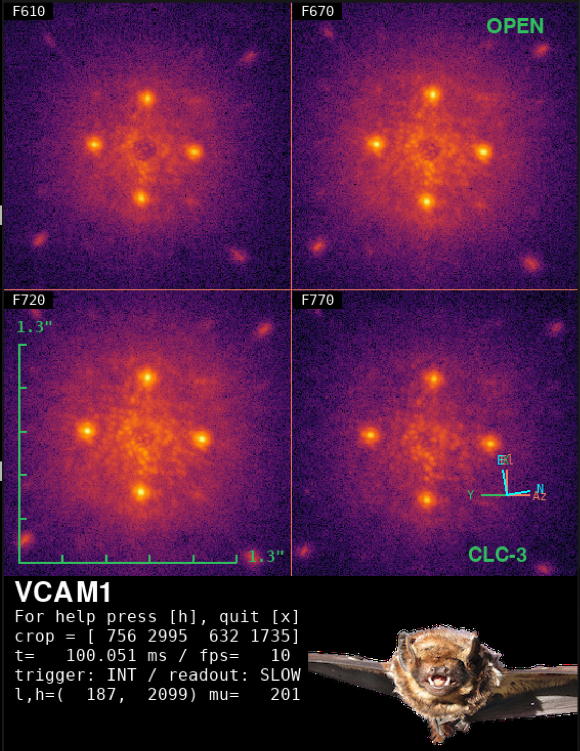
\includegraphics[width=0.95\columnwidth]{figures/vcam1_viewer.png}
    \caption{The custom \texttt{PyGame} camera viewer for VCAM1. Shown is a screenshot from on-sky observations on \formatdate{7}{7}{2023} in multiband imaging mode with the \SI{59}{\mas} coronagraph.}
    \label{fig:vcam1}
\end{figure}
% \tablenotetext{a}{The bat in the camera viewers is the Hawai`ian Ope`ape`a.}
